\documentclass{article}
\usepackage{tikz}
\usetikzlibrary{intersections}
\usetikzlibrary{positioning}
\usetikzlibrary{backgrounds}
\usetikzlibrary{fit}
\usetikzlibrary{through}

\begin{document}
We are working on 
\begin{tikzpicture}
\draw (-1.5, 0) -- (1.5, 0);
\draw (0, -1.5) -- (0, 1.5);
\end{tikzpicture}

\tikz \draw (-1.5, 0) -- (1.5, 0) -- (0, -1.5) -- (0, 1.5);

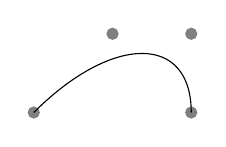
\begin{tikzpicture}
\filldraw [gray] (0, 0) circle [radius = 2pt] (1, 1) circle [radius = 2pt] (2, 1) circle [radius = 2pt] (2, 0) circle [radius = 2pt];
\draw (0, 0) .. controls (1, 1) and (2, 1) .. (2, 0);
\end{tikzpicture}

\tikz \draw (0, 0) circle [radius = 10pt];

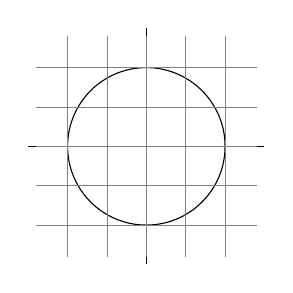
\begin{tikzpicture}
\draw (-1.5, 0) -- (1.5, 0);
\draw (0, -1.5) -- (0, 1.5);
\draw (0, 0) circle [radius = 1cm];
\draw[step = 0.5cm, very thin, gray] (-1.4, -1.4) grid (1.4, 1.4);
\end{tikzpicture}

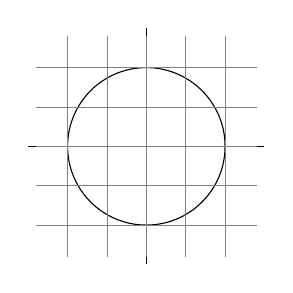
\begin{tikzpicture}
\draw (-1.5, 0) -- (1.5, 0);
\draw (0, -1.5) -- (0, 1.5);
\draw (0, 0) circle [radius = 1cm];
\draw[step = 0.5cm, help lines] (-1.4, -1.4) grid (1.4, 1.4);
\end{tikzpicture}

\begin{tikzpicture}[Karl's grid/.style = {help lines, color = #1!50}, Karl's grid/.default = blue]
\draw[Karl's grid] (0, 0) grid (1.5, 2);
\draw[Karl's grid = red] (2, 0) grid (3.5, 2);
\end{tikzpicture}

A sine \tikz \draw[x = 1ex, y = 1ex] (0, 0) sin (1.57, 1); curve

\tikz \draw[x = 1.57ex, y = 1ex] (0, 0) sin (1, 1) cos (2, 0) sin (3, -1) cos (4, 0);

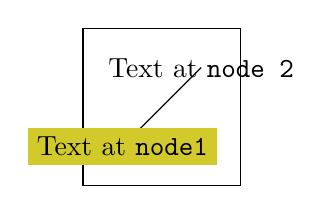
\begin{tikzpicture}
\draw (0, 0) rectangle (2, 2);
\draw (0.5, 0.5) node [fill = yellow!80!black] {Text at \verb!node1!} -- (1.5, 1.5) node {Text at \verb!node 2!};
\end{tikzpicture}

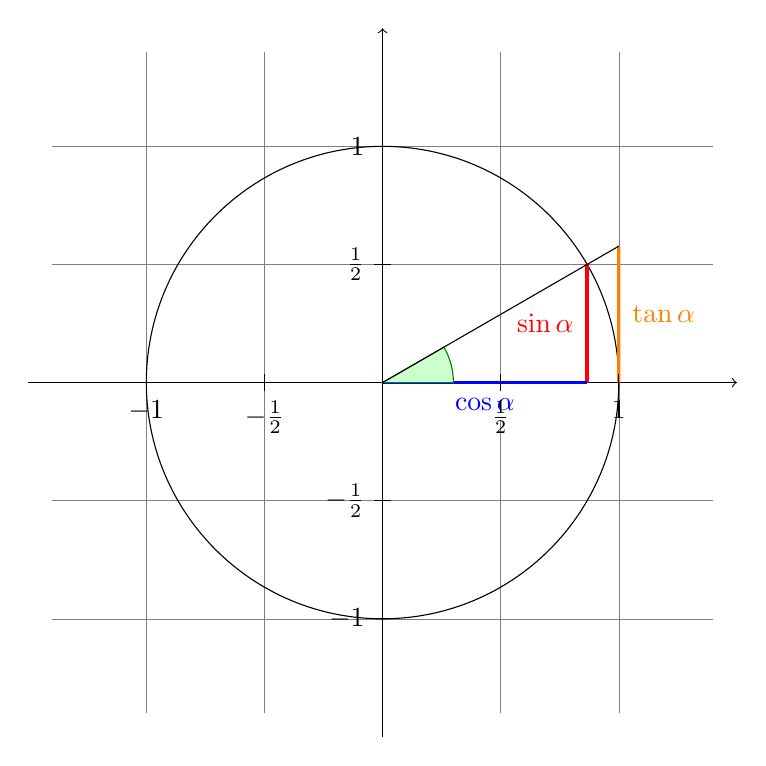
\begin{tikzpicture}[scale = 3]
%\clip (-0.1, -0.2) rectangle (1.1, 0.75);
\draw[step = 0.5, gray, very thin] (-1.4, -1.4) grid (1.4, 1.4);
\draw[->] (-1.5, 0) -- (1.5, 0) coordinate (x axis);
\draw[->] (0, -1.5) -- (0, 1.5) coordinate (y axis);
\draw (0, 0) circle [radius = 1cm];
\draw[very thick, red] (30:1cm) -- node[left = 1pt, fill = white] {$\sin\alpha$} (30:1 cm |- x axis);
\draw[very thick, blue] (30:1 cm |- x axis) -- node[below = 2pt, fill = white] {$\cos\alpha$} (0, 0);
\filldraw[fill = green!20!white, draw = green!50!black] (0, 0) -- (3mm, 0mm) arc [start angle = 0, end angle = 30, radius = 3mm] -- cycle;
\path [name path = upward line] (1, 0) -- (1, 1);
\path [name path = sloped line] (0, 0) -- (30:1.5cm);
\draw [name intersections = {of = upward line and sloped line, by = x}] [very thick, orange] 
(1, 0) -- node[right = 1pt, fill = white] {$\tan\alpha$} (x);
\draw (0, 0) -- (x);
\foreach \x/\xtext in {-1, -0.5/-\frac{1}{2}, 0.5/\frac{1}{2}, 1} \draw (\x cm, 1pt) -- (\x cm, -1pt) node[below] {$\xtext$};
\foreach \y/\ytext in {-1, -0.5/-\frac{1}{2}, 0.5/\frac{1}{2}, 1} \draw (1pt, \y cm) -- (-1pt, \y cm) node[left] {$\ytext$};
\end{tikzpicture}

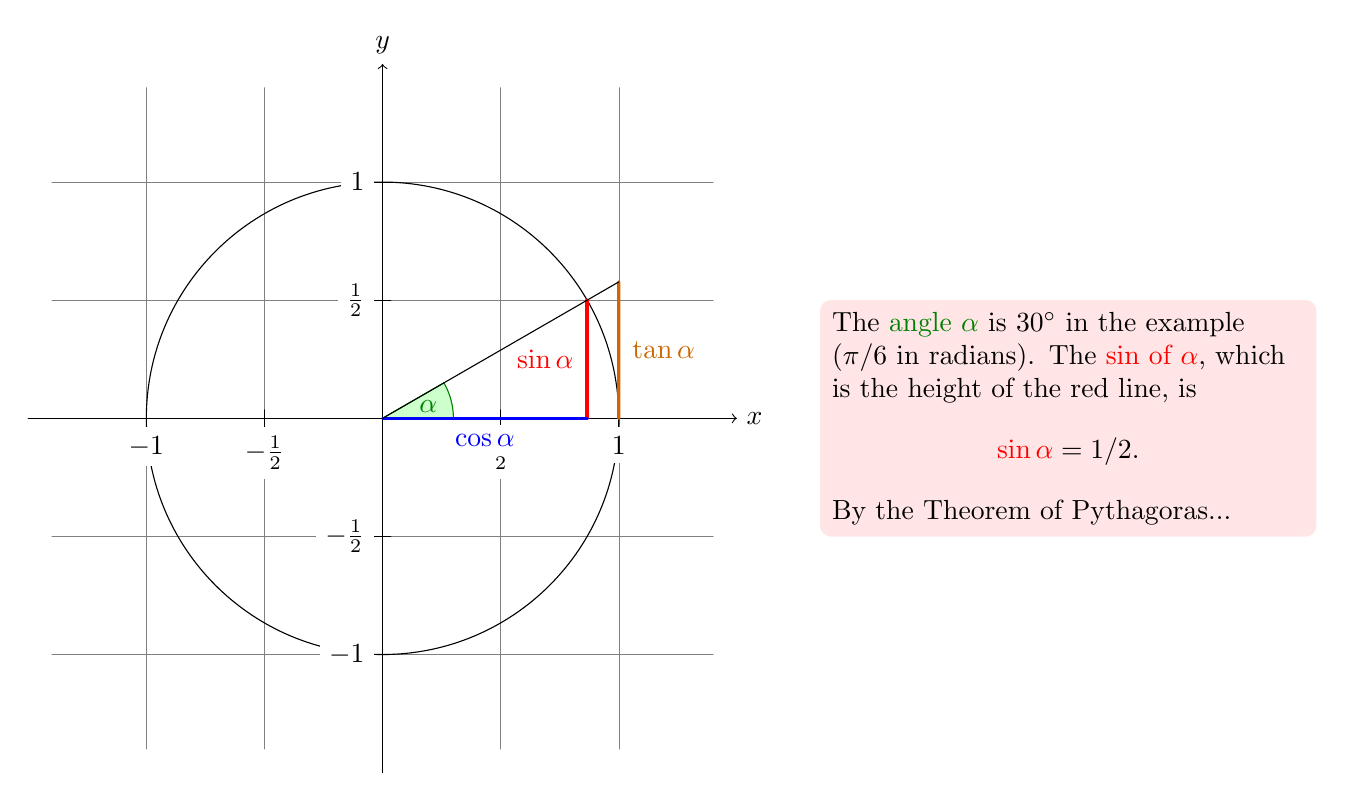
\begin{tikzpicture}
[scale = 3, line cap = round, 
axes/.style =, 
important line/.style = {very thick}, 
information text/.style = {rounded corners, fill = red!10, inner sep = 1ex}]

\colorlet{anglecolor}{green!50!black}
\colorlet{sincolor}{red}
\colorlet{tancolor}{orange!80!black}
\colorlet{coscolor}{blue}

\draw[help lines, step = 0.5 cm] (-1.4, -1.4) grid (1.4, 1.4);
\draw (0, 0) circle [radius = 1cm];

\begin{scope}[axes]
\draw[->] (-1.5, 0) -- (1.5, 0)  node[right] {$x$} coordinate (x axis);
\draw[->] (0, -1.5) -- (0, 1.5) node[above] {$y$} coordinate (y axis);
\foreach \x/\xtext in {-1, -0.5/-\frac{1}{2}, 0.5/\frac{1}{2}, 1} \draw (\x cm, 1pt) -- (\x cm, -1pt) node[below, fill = white] {$\xtext$};
\foreach \y/\ytext in {-1, -0.5/-\frac{1}{2}, 0.5/\frac{1}{2}, 1} \draw (1pt, \y cm) -- (-1pt, \y cm) node[left, fill = white] {$\ytext$};
\end{scope}

\filldraw[fill = green!20!white, draw = anglecolor] (0, 0) -- (3mm, 0mm) arc [start angle = 0, end angle = 30, radius = 3mm] -- cycle;
\draw (15:2mm) node[anglecolor] {$\alpha$};

\draw[important line, sincolor] (30:1cm) -- node[left = 1pt, fill = white] {$\sin\alpha$} (30:1 cm |- x axis);
\draw[important line, coscolor] (30:1 cm |- x axis) -- node[below = 2pt, fill = white] {$\cos\alpha$} (0, 0) ;

\path [name path = upward line] (1, 0) -- (1, 1);
\path [name path = sloped line] (0, 0) -- (30:1.5cm);
\draw [name intersections = {of = upward line and sloped line, by = x}] [important line, tancolor] 
(1, 0) -- node[right = 1pt, fill = white] {$\tan\alpha$} (x);
\draw (0, 0) -- (x);

\draw[xshift = 1.85 cm] node[right, text width = 6cm, information text] {
The {\color{anglecolor} angle $\alpha$} is $30^\circ$ in the example ($\pi/6$ in radians). The {\color{sincolor} sin of $\alpha$}, which is the height of the red line, is 
$$
{\color{sincolor} \sin\alpha} = 1/2.
$$
By the Theorem of Pythagoras...
};
\end{tikzpicture}

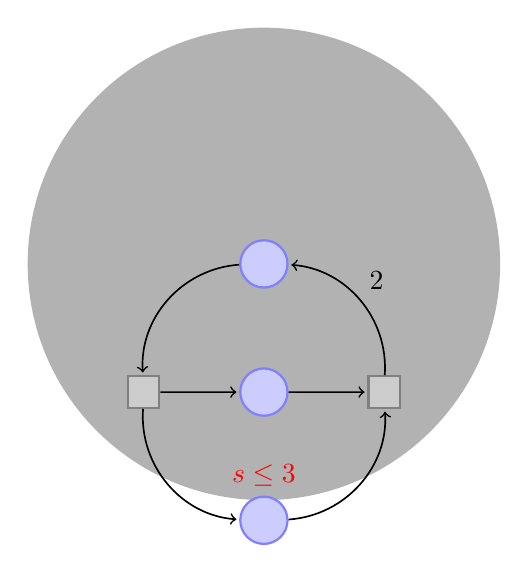
\begin{tikzpicture}
[bend angle = 45, 
pre/.style = {<-, shorten <=1pt, semithick}, 
post/.style = {->, shorten >=1pt, semithick}, 
every label/.style = {red}, 
scale = 3,  
place/.style = {circle, draw = blue!50, fill = blue!20, thick, minimum size = 6mm}, 
transition/.style = {rectangle, draw = black!50, fill = black!20, thick, minimum size = 4mm}]

\node[place] (waiting) {};
\node[place] (critical) [below = of waiting] {};
\node[place] (semaphore) [below = of critical, label = above: $s\le 3$] {};
\node[transition] (leave critical) [right = of critical] {}
edge[pre] (critical)
edge[post, bend right] node[auto, swap] {2} (waiting)
edge[pre, bend left] (semaphore);
\node[transition] (enter critical) [left = of critical] {}
edge[post] (critical) 
edge[pre, bend left] (waiting)
edge[post, bend right] (semaphore);

\begin{scope}[on background layer]
\fill[black!30] (0, 0) circle [radius = 1cm];%\node[fill = black!30, fit = (waiting) (critical) (semaphore) (leave critical) (enter critical)] {};
\end{scope}
\end{tikzpicture}


\begin{tikzpicture}
\draw[->] (0, 0) -- (3, 0) node[above, text width = 3cm, align = center, midway] {test};
\end{tikzpicture}

\begin{tikzpicture}
\draw[->] (0, 0) -- node[above, text width = 3cm, align = center] {test} (3, 0);
\end{tikzpicture}


\begin{tikzpicture}
\draw[->] (0, 0) -- (3, 0) node[above, text width = 3cm, align = center] {test};
\end{tikzpicture}

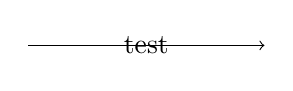
\begin{tikzpicture}
\draw[->] (0, 0) -- (3, 0) node[midway] {test};
\end{tikzpicture}

\tikz \draw[->] (0cm, 1em) -- (3cm, 1em) node[midway] {D};


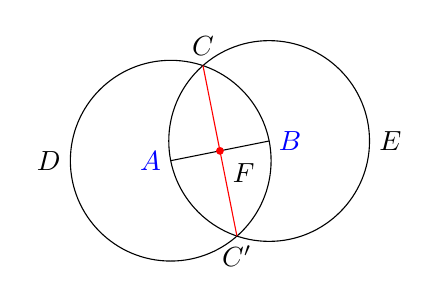
\begin{tikzpicture}
\coordinate[label = left:\textcolor{blue}{$A$}] (A) at (0, 0);
\coordinate[label =  right:\textcolor{blue}{$B$}] (B) at (1.25, 0.25);
\draw[name path = A--B] (A) -- (B);

\node[name path = D, draw, circle through = (B), label = left:$D$] (D) at (A) {};
\node[name path = E, draw, circle through = (A), label = right:$E$] (E) at (B) {};

\path[name intersections = {of = D and E, by = {[label = above:$C$]C, [label = below:$C'$]C'}}];

\draw[name path = C--C', red] (C) -- (C');

\path[name intersections = {of = A--B and C--C', by = F}];
\node[fill = red, circle, inner sep = 1pt, label = below right:$F$] at (F) {};

\end{tikzpicture}

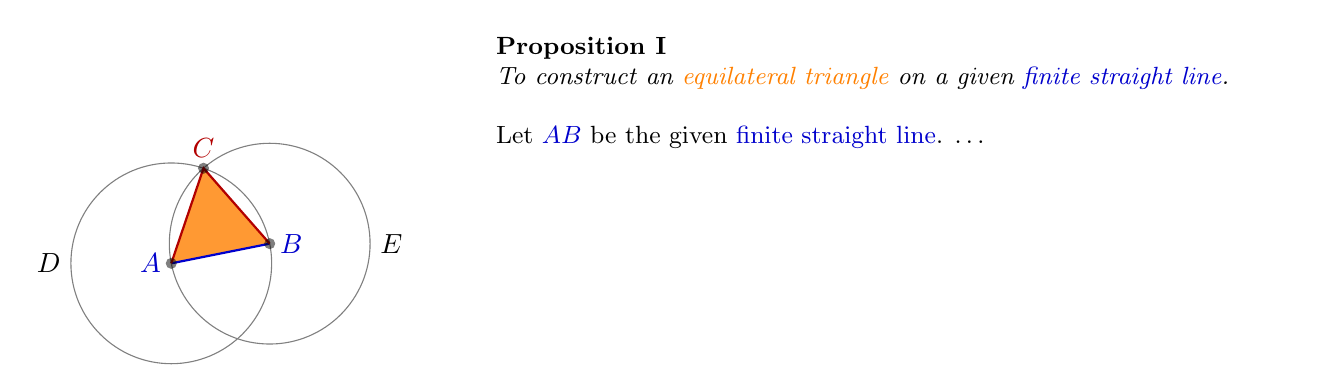
\begin{tikzpicture}[thick, help lines/.style = {thin, draw = black!50}]
\def\A{\textcolor{input}{$A$}}
\def\B{\textcolor{input}{$B$}}
\def\C{\textcolor{output}{$C$}}
\def\D{$D$}
\def\E{$E$}

\colorlet{input}{blue!80!black}
\colorlet{output}{red!70!black}
\colorlet{triangle}{orange}

\coordinate[label = left:\A] (A) at (0, 0);
\coordinate[label = right:\B] (B) at (1.25, 0.25);
\draw[input] (A) -- (B);

\node[name path = D, help lines, draw,, label = left:\D, circle through = (B)] (D) at (A) {};
\node[name path = E, help lines, draw, label = right:\E, circle through = (A)] (E) at (B) {};

\path[name intersections = {of = D and E, by = {[label = above:\C]C}}];

\draw[output] (A) -- (C) -- (B);

\foreach \point in {A, B, C} \fill[black, opacity = 0.5] (\point) circle (2pt);

\begin{pgfonlayer}{background}
\fill[triangle!80] (A) -- (C) -- (B) -- cycle;
\end{pgfonlayer}

\node[below right, text width = 10cm, align = justify] at (4, 3) {
\small\textbf{Proposition I}\par
\emph{To construct an \textcolor{triangle}{equilateral triangle}
on a given \textcolor{input}{finite straight line}.}
\par\vskip1em
Let \A\B\ be the given \textcolor{input}{finite straight line}. \dots
};
\end{tikzpicture}


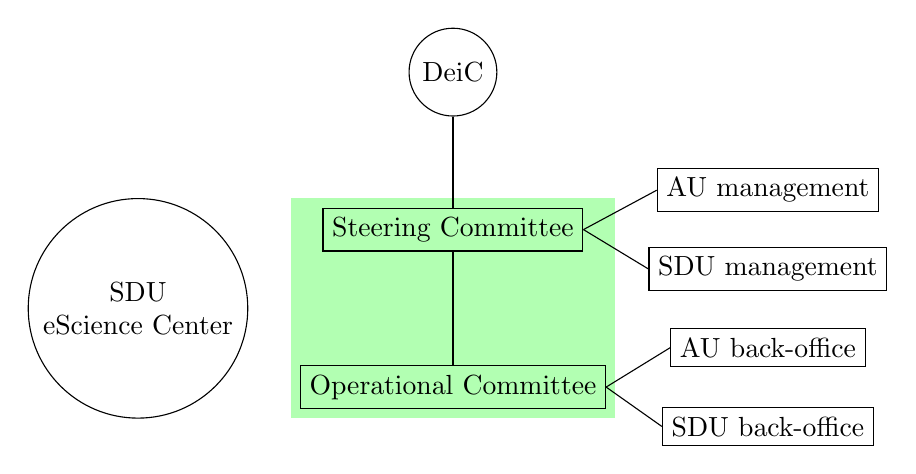
\begin{tikzpicture}[
management/.style ={draw, rectangle}, 
backoffice/.style =, 
center/.style = {circle, align = center, draw}]

\node[draw, circle] (deic) at (0, 4) {DeiC};
\node[draw, rectangle] (steering) at (0, 2) {Steering Committee};
\node[draw, rectangle] (operation) at (0, 0) {Operational Committee};
\node[draw, rectangle] (sdu backoffice) at (4, -0.5) {SDU back-office};
\node[draw, rectangle] (au backoffice) at (4, 0.5) {AU back-office};
\node[management] (sdu management) at (4, 1.5) {SDU management};
\node[management] (au management) at (4, 2.5) {AU management};
\node[center] (escience) at (-4, 1) {SDU\\eScience Center};

\draw (steering.east) -- (au management.west);
\draw (steering.east) -- (sdu management.west);
\draw (operation.east) -- (au backoffice.west);
\draw (operation.east) -- (sdu backoffice.west);
\draw (operation) -- (steering);
\draw (steering) -- (deic);

\begin{scope}[on background layer]
\node[fill = green!30, fit = (operation) (steering)] (back) {};
\end{scope}

\end{tikzpicture}



\end{document}